\chapter{Language sample}\label{sec:2}

  This chapter describes the language sample used in the study. In \sectref{sec:2.1} I discuss general issues of language sampling and specific considerations for sampling in the current study. In \sectref{sec:2.2} I examine a previous typology of syllable structure complexity and propose a definition for a category of Highly Complex syllable structure. In \sectref{sec:2.3} I discuss the procedure underlying the construction of the language sample. In \sectref{sec:2.4} I present the language sample and describe its areal, genealogical, and sociolinguistic features. In \sectref{sec:2.5} I briefly discuss the general method of data collection.

\section{Language sampling}\label{sec:2.1}

  Crosslinguistic comparison is “the fundamental characteristic of typology” \citep[6]{Croft2003}. In order to make general statements about some linguistic property such as syllable complexity, it is necessary to examine the properties of and variation within that feature in a wide variety of languages. Today, linguists have access to a greater array of grammatical descriptions, corpora, and audiovisual materials than ever before. However, for many languages, reference materials are either not available or not descriptive enough for inclusion in most typological studies. Therefore researchers must rely on samples much smaller than the set of the 7,097 languages known to exist today (\citealt{SimonsFennig2018}). Because typology is a data-driven science, the issue of sampling -- that is, determining which languages will serve as data sources for addressing the question(s) at hand -- is critical in any study. The relative merits of different sampling techniques and methods of controlling for various types of bias have often been the subject of debate in the field (see \citealt{Bakker2011} for an overview of the relevant literature). 

  Before introducing the sample used in the current study, I discuss some of the known sources of bias in typological work. I also discuss the potential effect of these factors on investigating issues of syllable structure or phonology more generally.

\subsection{Common sources of bias in language sampling}\label{sec:2.1.1}

  The three most commonly discussed sources of bias in language sampling are \textit{genealogical}, \textit{areal}, and \textit{bibliographic} bias \citep{Bakker2011}. 

  A typological study may suffer from \textit{genealogical bias} if it includes data from related languages. This presents a potential confound in the interpretation of results, because similar patterns in related languages may not be independent of one another, but instead inherited from a common ancestor. Of all the sources of bias in language sampling, genealogical bias is perhaps the most discussed, and the one most explicitly controlled for. Strategies for minimizing this kind of bias include systematic stratification of the language sample itself at a particular time depth or level of genealogical classification (\citealt{Bell1978b,Maddieson1984,Dryer1989}), or postponement of sampling to post-hoc analysis, when the independence of the feature(s) under study can be determined at each taxonomic level within a language family \citep{Bickel2008}. In practice, though, most typological studies are based on small convenience samples which are heavily skewed towards large, well-known, and well-described language families. Language isolates, which account for up to one-third of known language families \citep{Campbell2016}, and smaller, lesser-known language families often go altogether unrepresented.

  Another bias which is often considered in constructing language samples is \textit{areal bias}, in which languages spoken in the same geographical and/or cultural area may have influenced one another through prolonged contact. The literature has long noted the existence of linguistic areas, in which languages from more than one family share sets of traits in common with each other but not with other related languages spoken outside the area (\citealt{AikhenvaldDixon2001a,Chirikba2008}). Attempts to minimize such bias include consideration of cultural areas in addition to genealogical affiliations in constructing a language sample, with the ideal sample containing no two languages from the same family or area \citep{Perkins1985}. But while traditional linguistic areas are relatively small and geographically delimited (e.g., the Balkan Sprachbund), studies of individual features have revealed even larger areas of linguistic convergence; e.g., North America has a higher prevalence of head-marking agreement strategies as compared to the rest of the world \citep{Dryer1989}. To minimize the effects of areal bias, Dryer proposes a method by which a language sample may be divided into five large continental areas (later refined to six, \citealt{Dryer1992}), which can be shown to be independent of one another along at least some typological measures.

  As many as two-thirds of spoken languages do not have reference materials which are thorough enough to be consulted in any but the most basic of typological surveys \citep[106]{Bakker2011}. As a result, virtually every language sample suffers from severe \textit{bibliographic bias}. The best documented languages in the world tend to correspond to those which, for whatever historical reason, have the greatest political, social, and economic power and wide geographic spread (e.g., English, Mandarin Chinese, Spanish, Arabic). Thus we find that bibliographic bias is genealogically and areally skewed, with small, less powerful language families and remote regions particularly underrepresented. The least documented language families in the world, for example, tend to be found in lowland New Guinea and parts of the Amazon region \citep{Hammarström2010}. Similar to, or perhaps a subset of, bibliographic bias is what Moreno Cabrera describes as the \textit{written language bias}. Most of the world’s languages do not have a written or standard form, and references for such languages often describe a specific dialect or ideolect. When languages do have a written or standard form, reference materials often describe that form. A result of this is that typological studies often compare data from “highly heterogeneous sources”: standardized, highly formal registers for written languages, and unstandardized, informal registers of ideolects for unwritten languages (2008: 118).

  All three of the sources of bias described above -- genealogical, areal, and bibliographic bias -- may complicate typological studies of syllable structure. As discussed in the introduction, the prevalence of particular consonant cluster patterns in Indo-European languages may skew general perceptions regarding the universality of these patterns. There are also clear areal asymmetries in the global distribution of syllable structure complexity. Languages with Simple syllable structure tend to be spoken near the equator \citep{Maddieson2013a}. Complex syllable structure has been described as a prominent areal feature of specific regions such as the Caucasus \citep{Chirikba2008} and the Pacific Northwest (\citealt{ThompsonKinkade1990}), though there is evidence that maximal syllable structure is more strongly associated with genealogical affiliation even within these linguistic areas (\citealt{NapoleãodeSouza2017}). Insofar as the global distribution of syllable structure complexity is genealogically and areally skewed, the issue of bibliographic bias is relevant. For example, underdocumented areas such as the New Guinea are known to have a higher than average proportion of languages with canonical (C)V syllable structure \citep{Maddieson2013a}.

\subsection{Other factors which may influence phonological structure and syllable complexity}\label{sec:2.1.2}
\subsubsection{{Population}}\label{sec:2.1.2.1}

  Speaker population may have an affect on language structure. It has been proposed that rare or linguistically marked structures, such as Object-initial basic word orders, are more likely to arise and persist in small speech communities \citep{Nettle1999a}. Lingua francas which have wide areal spreads and large speaker populations with many second-language speakers may be more vulnerable to simplificatory pressures than languages whose use is limited to small, close-knit communities (\citealt{Nettle1999b,LupyanDale2010}). These proposals suggest that simpler syllable structures may be found in languages with large speaker populations or in situations of heavy language contact. Recent research on emergent phonology in creoles does not necessarily support the latter claim: despite many claims to the contrary, a broad range of complex syllable patterns may occur in these languages \citep{Schramm2014}. Concerning other phonological properties, a positive correlation between phoneme inventory size and speaker population has been noted (\citealt{HayBauer2007}). Proposed motivations for this pattern, including founder effects analogous to those found in genetics \citep{Atkinson2011}, are controversial (\citealt{Bybee2011,MaddiesonEtAl2011,HunleyEtAl2012}, \textit{inter alia}).

\subsubsection{{Language} {endangerment}}\label{sec:2.1.2.2}

  Today, language diversity is in precipitous decline due to rapid social, economic, and environmental changes which have global reach. It has been projected that 84\% or more of today’s languages may be lost within the next century \citep[113-114]{Nettle1999b}. There is evidence that language vitality status may influence linguistic structure itself. Languages which are obsolescing (dying) -- currently about 13\% of all living languages (\citealt{SimonsFennig2018}) -- are known to undergo special kinds of structural change (see \citealt{Romaine2010} for a review of research on the structural effects of language obsolescence). In the phonological systems of obsolescing languages, it is common for distinctive contrasts to be leveled and for the regularity of phonological processes to break down. Attested effects of obsolescence on syllable structure include reduction and simplification of syllable margins (\citealt{Cook1989}, for obsolescing dialects of Chipewyan and Sarcee) and the deletion of entire unstressed syllables in certain word positions (\citealt{Mithun1989}, for Oklahoma Cayuga).

\subsubsection{{Ecological} {factors}}\label{sec:2.1.2.3}

  There is a growing body of work investigating the effect of ecological factors on language structure. Recent studies have explored the hypothesis that the sound systems of human languages may be adapted to features of the natural environment such as elevation, ambient temperature, density of vegetation, and ambient dessication (\citealt{Everett2013,MaddiesonCoupé2015,EverettEtAl2016,Everett2017}). Syllable structure has been a subject of particular focus in this research paradigm. A positive correlation between warm climates and the frequency of CV shapes in languages has been proposed to reflect the communication needs of an outdoor lifestyle, in which more sonorous elements of the speech signal may overcome environmental noise and large distances between speakers (\citealt{MunroeEtAl1996,FoughtEtAl2004}). Similarly, a negative correlation between density of vegetation and complex syllable structures may reflect the poor transmission qualities of higher frequency sounds (certain consonants and consonant clusters) in densely forested environments (\citealt{MaddiesonCoupé2015}).

\subsection{Specific considerations in the current study}\label{sec:2.1.3}

  \citet[106]{Bakker2011} states that “the construction of a sample should follow the precise formulation of the research questions one would like to answer on the basis of it”. Recall the two broad research questions motivating this study, presented in \xxref{ex:2.1}{ex:2.2}:

\ea\label{ex:2.1}
   \textit{Do languages with highly complex syllable structure share other phonetic and phonological characteristics such that this group can be classified as a linguistic type?}
\z

\ea\label{ex:2.2}
   \textit{How does highly complex syllable structure develop over time?}
\z

  These research questions, and their more specific formulations laid out in \chapref{sec:1}, necessitate a carefully constructed language sample. The first seeks to determine whether there are structural features correlated with highly complex syllable structure such that this phenomenon can be considered characteristic of a language type. For the purposes of gaining a thorough understanding of a language type, genealogical and areal diversity are important considerations in the construction of the sample. However, because this study does not aim to quantify the range or overall distribution of highly complex syllable structure, it is not necessary that the sample be genealogically \textit{balanced} in a systematic way. If quantitative analysis reveals crosslinguistically robust patterns of features correlated with syllable structure complexity, these can inform specific predictions about the evolution of highly complex syllable structure, addressing the second research question. Thus it may actually prove useful to have pairs of related languages with different syllable structure complexity in the sample. The effectiveness of the predictions can then be tested and qualitatively evaluated within these pairs, in which the structures are known to derive from the same origin at some point in the past.

  In order to test for correlations between syllable structure complexity and other structural features, typological bias \citep[12]{Comrie1989} must be built into the sample. That is, the languages of the sample must be deliberately chosen on the basis of their syllable patterns, so that features of languages with different syllable structure complexity may be compared against one another in a principled way to determine whether the hypothesized correlations exist and are crosslinguistically robust. An important question, then, is how syllable structure complexity is defined in the current study.

\section{Defining the categories of syllable structure complexity}\label{sec:2.2}

  Definitions of syllable structure complexity typically consider the size and phonological structure of the onset and coda.\footnote{{The size and structure of the nucleus may also be a consideration; cf. \citet{MaddiesonEtAl2013}.}} A classification which considers the size, shape, and differential behavior of onsets and codas, as well as dominant crosslinguistic patterns is given in \citet{Maddieson2013a}. While broad, this classification captures prevalent crosslinguistic trends in syllable structure and has proven useful in establishing correlations between syllable structure complexity and other features of language structure, such as consonant phoneme inventory size. In a 486-language survey, languages are classified into three categories according to the size and shape of their largest observed onsets and codas: 

\begin{description}
\item[Simple:] languages in which the onset is maximally one C, and codas do not occur.
\item[Moderately Complex:] languages in which the onset is maximally two Cs, the second of which is a liquid or a glide; and/or the coda consists of maximally one C.
\item[Complex:] languages in which the maximal onset is two Cs (the second of which is something other than a liquid or a glide) or larger than two Cs; and/or the maximal coda consists of two or more Cs.
\end{description}

The distribution of the 486 languages in Maddieson's survey according to these three categories can be found in \tabref{tab:2.1}.

\begin{table}
\begin{tabular}{lrr}
\lsptoprule
Syllable structure complexity & \textit{N} languages & Percentage\\\midrule
\textit{Simple} & 61 & 12.6\\
\textit{Moderately Complex} & 274 & 56.4\\
\textit{Complex} & 151 & 31.1\\
\lspbottomrule
\end{tabular}
\caption{\label{tab:2.1}Distribution of syllable structure complexity in languages of \citet{Maddieson2013a}.}
\end{table}

  In contrast to the tightly-defined Simple and Moderately Complex categories, the Complex category in \citet{Maddieson2013a} is diverse and open-ended. Languages in this category range from those whose most complex syllable is only a slight expansion on the Moderately Complex types -- such as a CVCC shape in which the first consonant of the coda is limited to a liquid or glide -- to those having far more complex structures involving up to eight consonants in a tautosyllabic cluster. In order to better understand the internal structure of the Complex category and the distribution of languages within it, I analyzed the size and shape of the maximal syllable structure of these 151 languages. A list of the languages in the sample, along with the references consulted, can be found in Appendix C. The distribution of these languages can be found in \tabref{tab:2.2}, according to the size of their maximal onsets and codas.\footnote{{Note that there are only 147 languages represented in \tabref{tab:2.2}. Four of the languages in the Complex category in \citet{Maddieson2013a} -- Canela-Krahô, Ik, Indonesian, and Yagaria -- have been reclassified as having Moderately Complex syllable structure in the current analysis.}}

\begin{table}
\begin{tabular}{*{8}{r}}
\lsptoprule
                 & \multicolumn{7}{c}{Onset}\\\cmidrule(lr){2-8}
 \multicolumn{1}{l}{Coda}     & \multicolumn{1}{c}{C} & \multicolumn{1}{c}{CC} & \multicolumn{1}{c}{CCC} & \multicolumn{1}{c}{CCCC} & \multicolumn{1}{c}{CCCCC} & \multicolumn{1}{c}{CCCCCC} & \multicolumn{1}{c}{CCCCCCC}\\\midrule
 {(none)}   & \cellcolor{lsLightGray} & 2 & 1 & 1 & - & - & -\\
 {C}        & \cellcolor{lsLightGray} & 23 & 9 & 1 & - & - & -\\
 {CC}       & 35 & 21 & 13 & 3 & - & - & -\\
 {CCC}      & 3 & 5 & 8 & 3 & - & - & -\\
 {CCCC}     & 4 & 2 & 4 & 2 & - & 1 & -\\
 {CCCCC}    & 1 & - & - & 1 & - & - & 1\\
 {CCCCCC}   & - & 1 & - & - & 1 & - & -\\
 {CCCCCCC}  & - & - & - & - & - & - & -\\
 {CCCCCCCC} & - & - & - & 1 & - & - & -\\
\lspbottomrule
\end{tabular}
\caption{\label{tab:2.2}Distribution of languages in Complex syllable structure category in \citet{Maddieson2013a}, according to the size of the most complex onset (columns) and coda (rows) structures observed in each language.}
\end{table}

  The visual distribution of the languages in \tabref{tab:2.2} is striking: most languages cluster toward the upper lefthand corner of the table. Over half of the languages in the Complex category have syllable-marginal clusters of two consonants or fewer; that is, onsets and codas no more complex than a sequence of two obstruents. Though onsets of up to seven consonants and codas of up to eight consonants occur, it is very rare for a language to have more than four consonants at either margin (7/147, 4.8\%).

  Another interesting property of the distribution in \tabref{tab:2.2} is that as cluster size increases, the crosslinguistic size asymmetry in onsets and codas appears to level out and then reverse. As discussed in \chapref{sec:1}, it is more common for a language to have complex onsets than complex codas. When smaller cluster sizes are considered, this pattern is clear even within the Complex category: languages which have three or more consonants in the onset are more common (50 languages) than languages which have these patterns in the coda (38 languages). However, when larger clusters are considered, we find that there is a reversal of the pattern: it is \textit{less} common for languages to have onsets of four or more consonants (15 languages) than to have codas of the same size (19 languages). Examining the specific patterns in more depth than what is presented in \tabref{tab:2.2}, it seems that this reversal occurs when clusters of three \textit{obstruents} are taken as the cutoff point: 24 languages have these, or more complex clusters, as an onset, and 26 languages have these, or more complex clusters, as a coda.

\subsection{Long sequences of obstruents: Tautosyllabic clusters or syllabic consonants?}\label{sec:2.2.1}

  The above point relates to an interesting feature of attested large onset and coda patterns, also mentioned in \chapref{sec:1}, which is that many of these structures do not exhibit the sonority-related sequencing restrictions and contours that are so common of languages with smaller onsets and codas. It is not unusual to observe tautosyllabic clusters consisting entirely of obstruents in languages with large onsets or codas \xxref{ex:2.3}{ex:2.4}:

\ea\label{ex:2.3}
\etriple{Cocopa}{Cochimi-Yuman}{USA, Mexico}

  \textit{pʂt͡ʃʔa\'{} ːw}\todo{check diacritics}

  ‘I hang up several (things)’

  \citep[36]{Crawford1966}
\z

\ea\label{ex:2.4}
\etriple{Itelmen}{Chukotko-Kamchatkan}{Russia}

  \textit{qsaɬtxt͡ʃ}

  ‘Follow!’

  (\citealt{GeorgVolodin1999}: 44)
\z

  Thus a common characteristic of the more extreme cases of Complex syllable structure is the presence of long sequences of obstruents. This phenomenon can also be found in Tashlhiyt, a language which is classified as having Complex syllable structure, but which descriptions list as having only simple \citep{Ridouane2008} or maximally biconsonantal (\citealt{PuechLouali1999}) onsets and codas. Because the language also has syllabic obstruents, it is possible to find words without vowels which consist entirely of voiceless obstruents (\ref{ex:2.5}a--b):

\ea\label{ex:2.5}
\etriple{Tashlhiyt}{Afro-Asiatic}{Morocco}
\ea  \textit{tfsχt}\\
\glt ‘you cancelled’

\ex  \textit{tftχtstː}\\
\glt ‘you rolled it (\textsc{f})’

  \citep[95]{Ridouane2002}
\z
\z

  There is evidence in the literature that word-initial \textit{onset clusters} and word-initial \textit{consonant sequences with syllabic obstruents} exhibit different gestural timing patterns between the rightmost consonant and vowel. \citet{GoldsteinEtAl2007} instrumentally investigated the predictions of a coupled oscillator model of syllable structure for these two different kinds of word-initial sequences. In Georgian, the timing lag between gestures associated with the rightmost consonant and the vowel decreased with larger word-initial consonant sequences, in line with the model’s predictions for onset clusters. Thus word-initial consonant sequences, such as that in \textit{t͡s’k’ɾiala} ‘shiny clean,’ can be interpreted as syllable onsets in Georgian. In Tashlhiyt, no such pattern was found with increasingly larger word-initial consonant sequences; that is, the instrumental evidence suggested that only the consonant immediately preceding the vowel was coupled to it. Thus the initial sequence in \textit{tsmun} ‘\textsc{3fs}-\textsc{caus}-accompany’ was interpreted as being syllabified as [ts.mun]. These results, expanded and confirmed by \citet{HermesEtAl2011}, lend support to the analysis of Tashlhiyt as having simple onsets and nucleus patterns which include syllabic obstruents, rather than large onset clusters.

  While the results summarized above suggest that onset clusters and word-initial consonant sequences with syllabic consonants are categorically different structures in terms of articulation, the situation is actually more complex than that. The Georgian data in \citet{GoldsteinEtAl2007} was from two speakers, but only one speaker showed the expected effect. The other speaker had timing patterns which more closely resembled the Tashlhiyt pattern. An examination of this speaker’s productions revealed the regular presence of an ”epenthetic” vowel between [k’] and [ɾ] in \textit{k'ɾiali} ‘glitter’ and \textit{t͡s’k’ɾiala} ‘shiny clean.’ When epenthesis occurred, the decreased timing lag between the rightmost consonant and vowel was not observed; that is, the word-initial sequence of consonants was split by a syllable boundary. The authors note that epenthesis occurred in the speech of both Georgian speakers, but not always in the same forms. However, when epenthesis did occur, it was in very specific phonological environments: when the place of articulation for C\textsubscript{1} was more posterior than that of C\textsubscript{2}. Setting aside the issue of vowel epenthesis for now,\footnote{{The issue of vowel epenthesis is an important one which has obvious implications for the analysis of syllable structure; this will be discussed further in \sectref{sec:3.2.2}.}} an interesting finding from \citet{GoldsteinEtAl2007} is that both timing patterns may occur for the same word-initial sequence in the same language.

  A related observation regarding large tautosyllabic clusters and syllabic obstruents is that some languages are analyzed as having both in their canonical syllable structure. For example, \citet{Crawford1966} analyzes Cocopa as having large onset clusters, such as [pʂt͡ʃʔ] in \REF{ex:2.3} above. In addition to these, he proposes that some unstressed syllables can be entirely consonantal, consisting of “an onset only or of an onset and a coda with a predictable ‘murmur’ vowel following the onset as phonetic peak” (1966: 34). For example, \textit{pt͡ʃxmuka\'{} p} ‘he embraced her’ is syllabified as [p\textsuperscript{i}.t͡ʃx\textsuperscript{a}.mu.ka\'{} p]\todo{check diacritics}
  (1966: 43; quality of ”murmur” vowel determined by environment). Patterns of the latter sort occur for specific consonantal combinations in Cocopa, much like the Georgian patterns described above. 

  There are also a number of languages which are analyzed by one author as having large tautosyllabic clusters, and by another as having simpler syllable margins but also syllabic obstruents. \citet{Hoard1978} gives several examples of languages from the Pacific Northwest which had previously been analyzed as having large onsets and/or codas but might be better thought of as having smaller syllable margins in addition to syllabic stops and affricates (e.g., Quileute, Puget Salish, and Nez Perce). Hoard bases his analyses on impressionistic transcriptions, considering syllables to reflect “the number of audible pulses” in the form which are delineated by “relative separation or detachment” from other segments or groups of segments (1978: 59-60). Similar disagreements of analysis can be found for Yine (Arawakan; \citealt{Matteson1965,Lin1997,Hanson2010}). Perhaps these languages are like Georgian and Cocopa above, in which different timing patterns may be produced by different speakers or for different consonant combinations. Without experimental data it is difficult to say whether one or both analyses are appropriate. What is clear, however, is that it is not uncommon for the same language, when exhibiting long sequences of consonants (especially obstruents) at word margins, to be alternately described as having large tautosyllabic clusters and/or syllabic obstruents. For this reason I argue that it is appropriate to group languages of both types together in the current study.

  The above approach also has some support in instrumental findings in the literature regarding the articulatory properties of consonantal nuclei. \citet{PouplierBeňuš2011} found that for syllabic liquids in Slovak, the kinematic properties of the consonantal gestures did not undergo consistent changes in nucleus position. The authors conclude that in this respect, syllables with consonantal nuclei behave like consonant clusters. According to other instrumental measures, syllabic liquids exhibit timing and gestural coordination relationships with adjacent consonants which are reminiscent of those found in onset or coda clusters, but still distinct from those found in both non-syllabic consonant clusters and vocalic nuclei. Similarly, \citet{FougeronRidouane2008} found that /k/ in Tashlhiyt does not undergo consistent acoustic or articulatory changes when syllabic. However, it does exhibit consistent and stable patterns of temporal alignment and coordination relationships with flanking consonants which are, as noted in the discussion of \citet{GoldsteinEtAl2007} above, similar to those expected for onset-nucleus-coda patterns. Thus the instrumental evidence point to syllabic consonants as phenomena which exhibit some of the coordination properties of vocalic nuclei while maintaining articulatory properties of non-syllabic consonants.

\subsection{Highly Complex syllable structure: A definition}\label{sec:2.2.2}

  Motivated by all of the observations above -- the distribution of languages in \tabref{tab:2.2}, three-obstruent clusters as the locus of the weakening of the onset/coda asymmetry, and the similar patterns observed in languages with large tautosyllabic obstruent clusters and those with syllabic obstruents -- I define Highly Complex syllable structure as follows:

\begin{description}
\item[Highly Complex:] languages in which the maximal onset or coda consists of three obstruents, or four or more Cs of any kind; and/or in which syllabic obstruents occur, resulting in word-marginal sequences of three or more obstruents.
\end{description}

  \tabref{tab:2.3} shows how the 486 languages in \citet{Maddieson2013a} are distributed with the addition of the Highly Complex category as defined above. The definition of the Complex category is adjusted accordingly, and the Simple and Moderately Complex categories are defined as in the previous work.

\begin{table}
\begin{tabular}{lrr}
\lsptoprule
Syllable structure complexity & {\textit{N}} {languages} & {Percentage}\\\midrule
\textit{Simple} & 61 & 12.6\\
\textit{Moderately Complex} & 278 & 57.2\\
\textit{Complex} & 110 & 22.6\\
\textit{Highly Complex} & 37 & 7.6\\
\lspbottomrule
\end{tabular}
\caption{\label{tab:2.3}A reanalysis of the data in \citet{Maddieson2013a}, with the added category of Highly Complex as defined in the current work.}
\end{table}

  While the structural divisions between the syllable structure complexity categories are not evenly distributed, they capture predominant crosslinguistic patterns and serve the specific aims of the current study. These categories provide a four-point scale by which syllable structure complexity can be correlated with other structural features. The Highly Complex category is also defined in such a way as to include the extreme end of the syllable structure complexity cline, but not so narrowly as to introduce extreme genealogical and areal bias into this group. This will allow for meaningful examination, both quantitative and qualitative, of the characteristics of this group of languages.

\section{Constructing the language sample}\label{sec:2.3}

  Three criteria shaped the design of the language sample for this study: (i) the size of the sample must be large enough for meaningful quantitative analysis, but small enough for in-depth qualitative analysis of the languages with highly complex syllable structure; (ii) the proportional representation of the four syllable structure complexity categories must be similar enough to allow for meaningful comparisons between the groups, and (iii) as per the discussion of bias in typological studies in \sectref{sec:2.1}, the sample should be both genealogically and areally diverse.

  In addressing (i), a sample of approximately 100 languages is appropriate. While this sample size is moderate for a phonological typology survey, it is comparable to those used in studies such as \citet{Bateman2007} and \citet{BybeeEasterday2019}, both of which have quantitative and qualitative components. Given the relative crosslinguistic rarity of languages in the Simple and Highly Complex categories (\tabref{tab:2.3}) and the skewed geographical and genealogical distribution of syllable structure complexity, meeting criteria (ii) and (iii) is a more difficult endeavor. In constructing the sample, an attempt was made to strike a reasonable balance between the ideal sample composition and these practical considerations. The resulting sample is described in the following section.
 
\section{Language sample for current study}\label{sec:2.4}

  The language sample includes 24 languages in the Simple category, 26 languages in the Moderately Complex category, 25 languages in the Complex category, and 25 languages in the Highly Complex category. Tables \ref{tab:2.4}--\ref{tab:2.7} list the languages of the sample by syllable structure complexity, geographical macro-area, and genealogical affiliation. A more detailed list which includes ISO 639-3 codes, speaker populations, and language endangerment and development status, can be found in Appendix A.

\begin{table}\small
\begin{tabularx}{\textwidth}{llQl}
\lsptoprule
{Region} & {Language} & {Top-level family} & {\textit{Subfamily}}\\\midrule
\multicolumn{4}{l}{\textsc{Africa}}\\
& {Hadza} & (isolate) & \\
& {Southern Grebo} & Atlantic-Congo & \textit{Volta-Congo}\\
& {Yoruba} & Atlantic-Congo & \textit{Volta-Congo}\\
& {Ma’di} & Central Sudanic & \textit{Moru-Madi}\\
& {Southern Bobo Madaré} & Mande & \textit{Western Mande}\\\midrule
\multicolumn{4}{l}{\textsc{Australia \& New Guinea}}\\
& {Savosavo} & (isolate) & \\
& {Grass Koiari} & Koiarian & \textit{Koiaric}\\
& {Rotokas} & North Bougainville & \textit{Rotokas-Askopan}\\
& {East Kewa} & Nuclear Trans New Guinea & \textit{Enga-Kewa-Huli}\\\midrule
\multicolumn{4}{l}{\textsc{North America}}\\
& {Towa} & Kiowa-Tanoan & \\
& {Pinotepa Mixtec} & Otomanguean & \textit{Eastern Otomanguean}\\
& {Ute} & Uto-Aztecan & \textit{Northern Uto-Aztecan}\\\midrule
\multicolumn{4}{l}{\textsc{South America}}\\
& {Urarina} & (isolate) & \\
& {Warao} & (isolate) & \\
& {Apurinã} & Arawakan & \textit{Southern Maipuran}\\
& {Murui Huitoto} & Huitotoan & \textit{Nuclear Witotoan}\\
& {Cavineña} & Pano-Tacanan & \textit{Tacanan}\\
& {Cubeo} & Tucanoan & \textit{Eastern Tucanoan}\\\midrule
\multicolumn{4}{l}{\textsc{Southeast Asia \& Oceania}}\\
& {Rukai (Budai dialect)} & Austronesian & \\
& {Maori} & Austronesian & \textit{Malayo-Polynesian}\\
& {Tukang Besi North} & Austronesian & \textit{Malayo-Polynesian}\\
& {Saaroa} & Austronesian & \textit{Tsouic}\\
& {Sichuan Yi} & Sino-Tibetan & \textit{Burmo-Qiangic}\\
& {Sumi Naga} & Sino-Tibetan & \textit{Kuki-Chin-Naga}\\
\lspbottomrule
\end{tabularx}
\caption{\label{tab:2.4.}Languages in \textbf{Simple} syllable structure category, by macro-area and genealogical affiliation.}
\end{table}




\begin{table}\small
\begin{tabularx}{\textwidth}{lQQQ}
\lsptoprule
Region & {Language} & {Top-level family} & {\textit{Subfamily}}\\\midrule
\multicolumn{4}{l}{\textsc{Africa}}\\
& {Kambaata} & Afro-Asiatic & \textit{Cushitic}\\
& {Ewe} & Atlantic-Congo & \textit{Volta-Congo}\\
& {Fur} & Furan & \\
& {Kanuri} & Saharan & \textit{Western Saharan}\\\midrule
\multicolumn{4}{l}{\textsc{Australia \& New Guinea}}\\
& {Maybrat} & Maybrat-Karon & \\
& {Kamasau} & Nuclear Torricelli & \textit{Marienberg}\\
& {Selepet} & Nuclear Trans New Guinea & \textit{Finisterre-Huon}\\
& {Alyawarra} & Pama-Nyungan & \textit{Arandic-Thura-Yura}\\\midrule
\multicolumn{4}{l}{\textsc{Eurasia}}\\
& {Kharia} & Austroasiatic & \textit{Munda}\\
& {Telugu} & Dravidian & \textit{South Dravidian}\\
& {Darai} & Indo-European & \textit{Indo-Iranian}\\
& {Tu} & Mongolic & \textit{Southern Periphery Mongolic}\\
& {Eastern Khanty} & Uralic & \textit{Khantyic}\\\midrule
\multicolumn{4}{l}{\textsc{North America}}\\ 
& {Karok} & (isolate) & \\
& {North Slavey} (Hare dialect) & Athabaskan-Eyak-Tlingit & \textit{Athabaskan-Eyak}\\
& {Kalaallisut} & Eskimo-Aleut & \textit{Eskimo}\\
& {Choctaw} & Muskogean & \textit{Western Muskogean}\\\midrule
\multicolumn{4}{l}{\textsc{South America}}\\ 
& {Carib} & Cariban & \textit{Guianan}\\
& {Imbabura Highland Quichua} & Quechuan & \textit{Quechua II}\\
& {Cocama-Cocamilla} & Tupian & \textit{Maweti-Guarani}\\\midrule
\multicolumn{4}{l}{\textsc{Southeast Asia \& Oceania}}\\
& {Pacoh} & Austroasiatic & \textit{Katuic}\\
& {Paiwan} & Austronesian & \\
& Kim Mun (Vietnam dialect) & Hmong-Mien & \textit{Mienic}\\
& {Atong} & Sino-Tibetan & \textit{Brahmaputran}\\
& {Cantonese} & Sino-Tibetan & \textit{Sinitic}\\
& {Lao} & Tai-Kadai & \textit{Kam-Tai}\\
\lspbottomrule
\end{tabularx}
\caption{\label{tab:2.5.}Languages in \textbf{Moderately Complex} syllable structure category, by macro-area and genealogical affiliation.}
\end{table}




\begin{table}\small
\begin{tabularx}{\textwidth}{lQQl}
\lsptoprule
{\textsc{Region}} & {Language} & {Top-level family} & {\textit{Subfamily}}\\\midrule
\multicolumn{4}{l}{\textsc{Africa}}\\
& {Mpade (Makari dialect)} & Afro-Asiatic & \textit{Chadic}\\
& {Jola-Fonyi} & Atlantic-Congo & \textit{North-Central Atlantic}\\
& {Lunda} & Atlantic-Congo & \textit{Volta-Congo}\\
& {Dizin (Central dialect)} & Dizoid & \\
& {Gaam} & Eastern Jebel & \\\midrule
\multicolumn{4}{l}{\textsc{Australia \& New Guinea}}\\
& {Mangarrayi} & Mangarrayi-Maran & \\
& {Nimboran} & Nimboranic & \\
& {Oksapmin} & Nuclear Trans New Guinea & \textit{Asman-Awyu-Ok}\\
& {Bardi} & Nyulnyulan & \textit{Western Nyulnyulan}\\
& {Ngarinyin} & Worrorran & \\\midrule
\multicolumn{4}{l}{\textsc{Eurasia}}\\
& {Basque (Central dialect)} & (isolate) & \\
& {Burushaski} & (isolate) & \\
& {Nivkh (West Sakhalin dialect)} & (isolate) & \\
& {Bashkir} & Turkic & \textit{Common Turkic}\\
& {Ket} & Yeniseian & \textit{Northern Yeniseian}\\\midrule
\multicolumn{4}{l}{\textsc{North America}}\\
& {Pech} & Chibchan & \\
& {Tzeltal (Aguacatenango dialect)} & Mayan & \textit{Core Mayan}\\
& {Lakota} & Siouan & \textit{Core Siouan}\\\midrule
\multicolumn{4}{l}{\textsc{South America}}\\
& {Kadiwéu} & Guaicuruan & \\
& {Mamaindê} & Nambiquaran & \textit{Nambikwara Complex}\\
& {Apinayé} & Nuclear-Macro-Je & \textit{Je}\\
& {Chipaya} & Uru-Chipaya & \\\midrule
\multicolumn{4}{l}{\textsc{Southeast Asia \& Oceania}}\\
& {Koho (Sre dialect)} & Austroasiatic & \textit{Bahnaric}\\
& {Lelepa} & Austronesian & \textit{Malayo-Polynesian}\\
& {Lepcha} & Sino-Tibetan & \textit{Himalayish}\\
\lspbottomrule
\end{tabularx}
\caption{\label{tab:2.6}Languages in \textbf{Complex} syllable structure category, by macro-area and genealogical affiliation.}
\end{table}




\begin{table}\small
\begin{tabularx}{\textwidth}{lQQQ}
\lsptoprule
{\textsc{Region}} & {Language} & {Top-level family} & {\textit{Subfamily}}\\\midrule
\multicolumn{4}{l}{\textsc{Africa}}\\
& {Tashlhiyt} & Afro-Asiatic & \textit{Berber}\\
& {Doyayo} & Atlantic-Congo & \textit{Volta-Congo}\\
& {Bench} & Ta-Ne-Omotic & \\\midrule
\multicolumn{4}{l}{\textsc{Australia \& New Guinea}}\\
& {Menya} & Angan & \textit{Nuclear Angan}\\
& {Kunjen (Oykangand dialect)} & Pama-Nyungan & \textit{Paman}\\
& {Alamblak} & Sepik & \textit{Sepik Hill}\\
& {Wutung} & Sko & \textit{Nuclear Skou-Serra-Piore}\\\midrule
\multicolumn{4}{l}{\textsc{Eurasia}}\\
& {Kabardian} & Abkhaz-Adyge & \textit{Circassian}\\
& {Itelmen} & Chukotko-Kamchatkan & \\
& {Albanian (Tosk dialect)} & Indo-European & \textit{Albanian}\\
& {Polish} & Indo-European & \textit{Balto-Slavic}\\
& {Georgian} & Kartvelian & \textit{Georgian-Zan}\\
& {Lezgian} & Nakh-Daghestanian & \textit{Daghestanian}\\\midrule
\multicolumn{4}{l}{\textsc{North America}}\\
& {Passamaquoddy-Maliseet} & Algic & \textit{Algonquian}\\
& {Cocopa} & Cochimi-Yuman & \textit{Yuman}\\
& {Mohawk} & Iroquoian & \textit{Northern Iroquoian}\\
& {Yakima Sahaptin} & Sahaptian & \textit{Sahaptin}\\
& {Thompson} & Salishan & \textit{Interior Salish}\\
& {Tohono O’odham} & Uto-Aztecan & \textit{Southern Uto-Aztecan}\\
& {Nuu-chah-nulth} & Wakashan & \textit{Southern Wakashan}\\\midrule
\multicolumn{4}{l}{\textsc{South America}}\\
& {Camsá} & (isolate) & \\
& {Yine} & Arawakan & \textit{Southern Maipuran}\\
& {Tehuelche} & Chonan & \textit{Continental Chonan}\\
& {Qawasqar} & Kawesqar & \textit{North Central Alacalufan}\\\midrule
\multicolumn{4}{l}{\textsc{Southeast Asia \& Oceania}}\\ 
& {Semai} & Austroasiatic & \textit{Aslian}\\
\lspbottomrule
\end{tabularx}
\caption{\label{tab:2.7}Languages in {Highly Complex} syllable structure category, by macro-area and genealogical affiliation.}
\end{table}

\subsection{Areal features of sample}\label{sec:2.4.1}

  The 100 languages are roughly evenly distributed among the six geographical macro-areas as defined by \citet{Dryer1989,Dryer1992}.\footnote{{The geographical macro-areas are specifically defined as follows (\citealt{Dryer1989}: 268; \citealt{Dryer1992}: 83, 133--135).} \textrm{\textbf{Africa}}\textrm{: continent of Africa, including Semitic languages of southwest Asia.} \textrm{\textbf{Australia \& New Guinea}}\textrm{: Australian continent and Melanesia, excluding Austronesian languages of Melanesia.} \textrm{\textbf{Eurasia}}\textrm{: Eurasian landmass, excluding Semitic and languages from families of southeast Asia as defined below, and including the Munda languages of Austroasiatic.} \textrm{\textbf{North America}}\textrm{: North American continent, including languages of Mexico, Mayan and Aztecan languages in Central America, and some branches of Chibchan-Paezan.} \textrm{\textbf{South America}}\textrm{: South American continent, including languages of Central America except Mayan and Aztecan languages, and some Chibchan-Paezan branches.} \textrm{\textbf{Southeast Asia \& Oceania}}\textrm{: Southeast Asian region, including all Sino-Tibetan, Tai-Kadai, Hmong-Mien, and Austroasiatic languages excluding Munda, and Oceania region (Austronesian languages).}} Africa, Australia \& New Guinea, North America, and South America are represented by 17 languages each. Two regions, Eurasia and Southeast Asia \& Oceania, are represented by 16 languages each. See \figref{fig:2.1} for a plotted map of the languages of the sample.

\begin{figure}
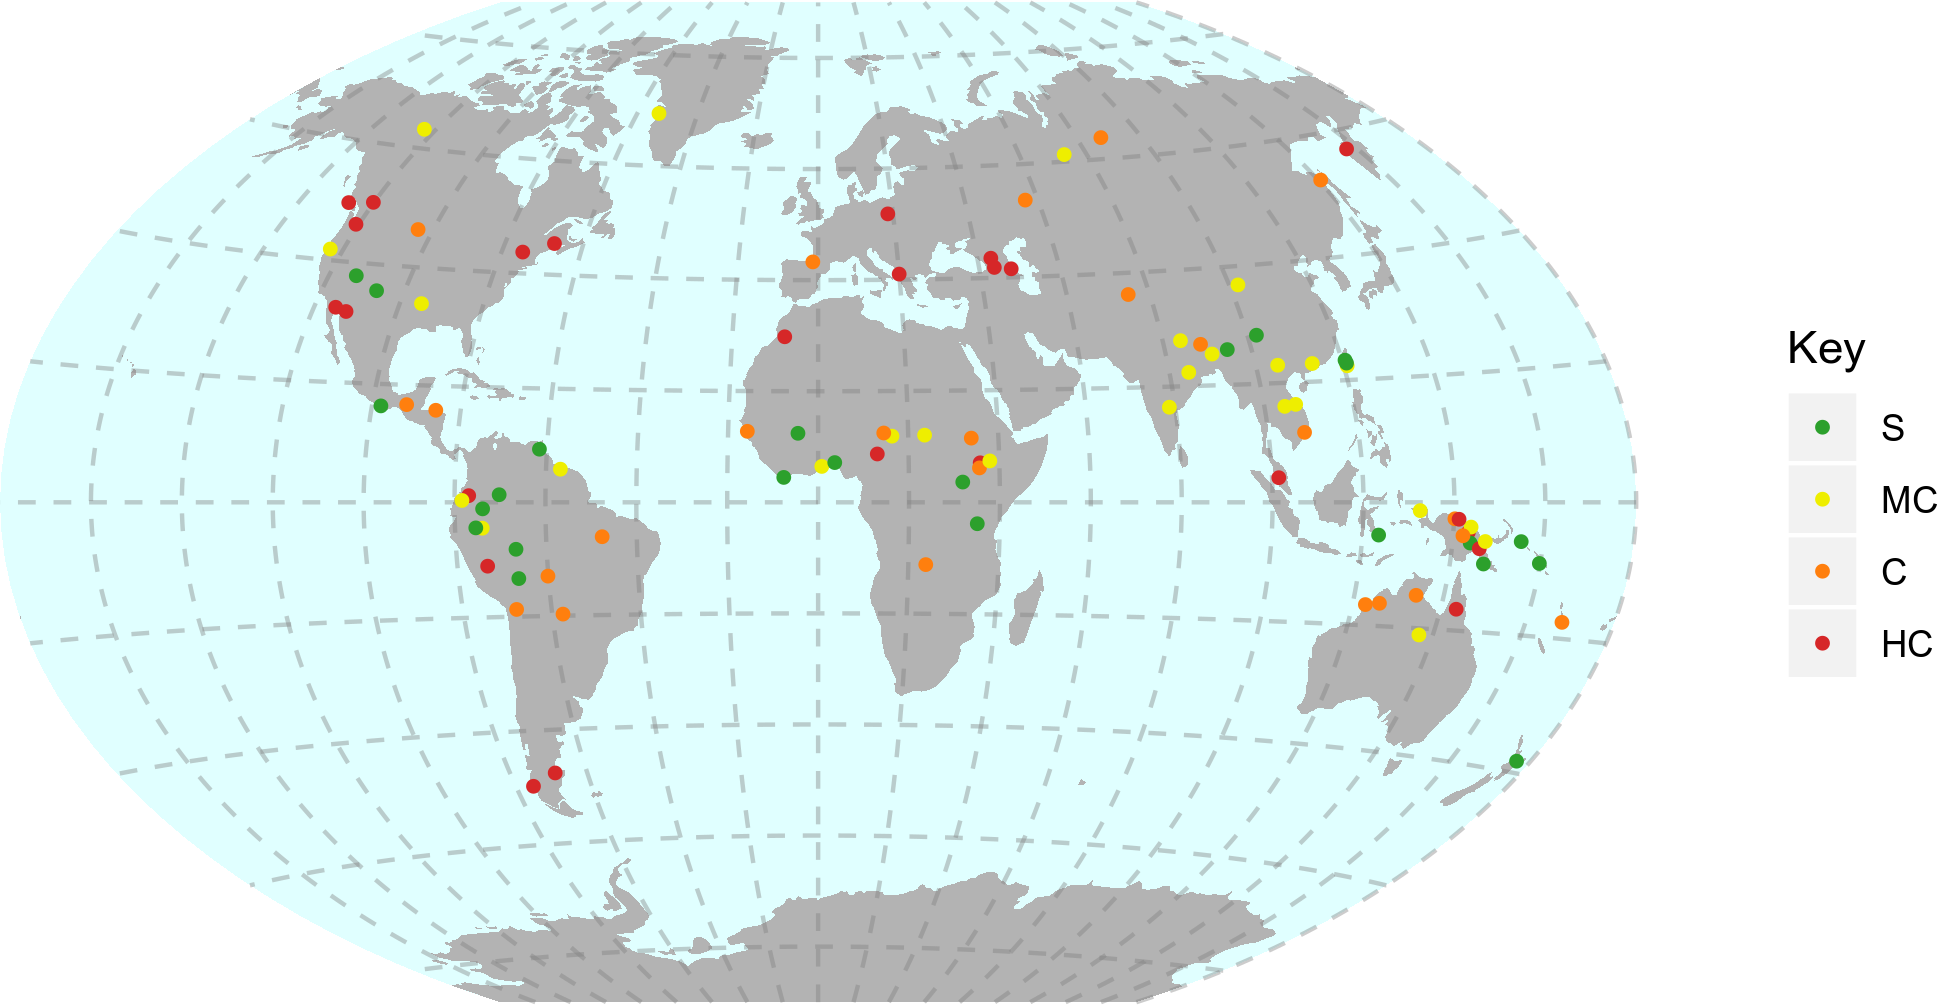
\includegraphics[width=\textwidth]{figures/fig21.png}
\caption{\label{fig:2.1}Geographic distribution of languages in the sample, with colors denoting syllable structure complexity. S\,=\,Simple, MC\,=\,Moderately Complex, C\,=\,Complex, HC\,=\,Highly Complex.}
\end{figure}

  There are some asymmetries in the areal representation of syllable structure complexity in the sample. In Eurasia, the Simple category is entirely unrepresented. In Southeast Asia \& Oceania, the Highly Complex category is represented by only one language. In North America, the Highly Complex category is relatively overrepresented, accounting for seven of the languages in that region.

\subsection{Genealogical features of sample}\label{sec:2.4.2}

  The 100 languages of the sample belong to 74 different language families.\footnote{{For genealogical affiliations, I use the classifications in Glottolog 3.3 \citep{HammarströmEtAl2018}.}} 64 of the language families are represented by one language each; this figure includes nine language isolates and many small and mid-sized families. Another three language families -- Arawakan, Pama-Nyungan, and Uto-Aztecan -- are represented in the sample by two languages each. All of the language families represented by more than two languages in the sample -- Afro-Asiatic, Atlantic-Congo, Austroasiatic, Austronesian, Indo-European, Nuclear Trans New Guinea, and Sino-Tibetan -- are within the top ten in the world by size in number of languages \citep{HammarströmEtAl2018}. Every attempt was made to maximize the diversity of subfamilies within the top-level families represented by more than one language in the sample. Subfamilies represented by more than one language are Volta-Congo (Atlantic-Congo family, five languages), Malayo-Polynesian (Austronesian family, three languages) and Southern Maipuran (Arawakan family, two languages). There are no pidgins or creoles in the sample.\footnote{{There is debate over whether Cocama-Cocamilla may be appropriately classified as a creole. While the language is typically classified as Tupi-Guaraní, it is quite divergent from other languages of the family in aspects of its phonology and morphosyntax, perhaps owing to factors of language contact. See  \citet{VallejosYopán2010} for a critical discussion of this topic.}}

  Most often, a language family is represented by only one language within a syllable structure complexity category. The Simple category is somewhat less genealogically diverse than the others, with only 19 families represented by the 24 languages.

  Recall from \sectref{sec:2.1.3} that an important feature of the language sample design is the inclusion of pairs of related languages with maximally different syllable structure complexities. This allows for hypotheses about the diachronic development of highly complex syllable structure to be tested at the local level. The sample includes five relevant pairs from five macro-areas: Ute (Simple) and Tohono O’odham (Highly Complex), both Uto-Aztecan from North America; Apurinã (Simple) and Yine (Highly Complex), both Arawakan from South America; Yoruba (Simple) and Lunda (Complex), both Atlantic-Congo from Africa; Darai (Moderately Complex) and Albanian (Highly Complex), both Indo-European from Eurasia; and Maori (Simple) and Lelepa (Complex), both Austronesian from Southeast Asia \& Oceania. Some pairs of languages are more closely related than others.\footnote{{The region of Australia \& New Guinea is not represented in these pair comparisons. The only family represented by more than one language in this region is Nuclear Trans New Guinea; however some of its subfamily classifications are controversial or not well demonstrated \citep{Pawley2005}.}}

\subsection{Sociolinguistic features of sample}\label{sec:2.4.3}

  Speaker population data and language vitality status classifications for the languages of the sample can be found in Appendix A.

  The L1 speaker populations for the languages of the sample vary widely, ranging from five for Tehuelche (Chonan, Patagonia) and Yakima Sahaptin (Sahaptian, Pacific Northwest) to 74,244,300 for Telugu (Dravidian, Southern India). In general, the languages in the Simple and Moderately Complex categories have larger speaker populations than those in the Complex and Highly Complex categories, though there are many exceptions to this trend. Of the 26 languages with fewer than 1,000 speakers, 18 of them have Complex or Highly Complex syllable structure, and half of the ten languages with fewer than 100 speakers have Highly Complex syllable structure. The prevalence of very smaller speaker populations among languages in these categories is no doubt related to the high concentration of these languages in geographical areas with high rates of language endangerment.

  The Expanded Graded Intergenerational Disruption Scale (EGIDS) is an assessment of language vitality developed by \citet{LewisSimons2010}, following work by \citet{Fishman1991}, UNESCO \citep{BrenzingerEtAl2003}, and others. It considers many different factors of language use, including rates and means of intergenerational transmission, domains of language use, and official recognition of the language. Using EGIDS as a starting point, Ethnologue (\citealt{SimonsFennig2018}) has developed a coarse-grained estimate of the relative development versus endangerment of languages. By this measure, languages are classified into categories according to their development/vitality status: Institutional, Developing, Vigorous, In Trouble, and Dying.\footnote{{The language development categories are defined as follows (\citealt{SimonsFennig2018}).} \textrm{\textbf{Institutional:} }\textrm{language has wide use in the home and community and official status at educational, provincial, national, and/or international levels.} \textrm{\textbf{Developing:} }\textrm{language is used in the home, community, and sometimes broader contexts, and in initial stages of developing a system of writing and standardization.}\textrm{ }\textrm{\textbf{Vigorous:} }\textrm{language is used in the home and community by speakers of all generations, but has not yet developed a system of graphization or standardization}\textrm{. }\textrm{\textbf{In Trouble:}} \textrm{language is currently in the process of losing intergenerational transmission, with the community shifting to other languages for daily use, but there are still speakers of child-bearing age.}\textrm{ }\textrm{\textbf{Dying:}} \textrm{language has lost intergenerational transmission entirely, all fluent speakers are above child-bearing age.}} Languages with robust vitality are more common in the Simple and Moderately Complex portions of the sample. The Complex and Highly Complex categories have the highest proportion of languages classified as Dying (6/25 languages in each category). It should be noted that in North America, which has perhaps the highest proportion of languages with Highly Complex patterns of all the macro-areas, rates of language endangerment and language loss are extreme. Ethnologue 21 classifies 237/254 (93\%) of the living languages spoken north of the US-Mexico border in North America as In Trouble or Dying (\citealt{SimonsFennig2018}). 

  The sociolinguistic features of the language sample lead to an interesting observation: highly complex syllable structure is a rare language feature by many different measures, including non-structural ones. As described in \chapref{sec:1}, highly complex phonotactic patterns are often treated as anomalies and theoretical outliers, especially when occurring in underdescribed non-European languages. A very small proportion of the world’s languages have structures of this kind. Many of the languages with these structures are found in parts of the world where language endangerment rates are particularly high, and have correspondingly small speaker populations. Thus highly complex syllable structure is a  marginalized pattern in theoretical, descriptive, historical, and social terms. This is all the more reason to dedicate a typological study to this linguistic feature.

\section{Data collection}\label{sec:2.5}

  The data used for this study was collected from published reference grammars, phonetic and phonological studies, and other relevant language descriptions. In a few cases, an expert researcher on the given language was additionally consulted. Data was collected with the guidance of coding sheets whose questions were designed to address the research questions and hypotheses of each chapter. As the methodology behind the coding of the data differs for each part of the study, it will be discussed separately within each chapter.

  Because the language references consulted were written in different time periods and reflect a variety of descriptive practices, they use diverse transcription standards. Using the phonetic descriptions of sounds in the language references, all phoneme inventories and phonetic and phonemic transcriptions have been transcribed using International Phonetic Alphabet (IPA) symbols. Where there is some ambiguity in interpreting the phonetic description provided by the source consulted, this has been noted in Appendix B. In the examples given in this chapter and throughout the book, non-IPA symbols have been replaced by their IPA equivalents.

